
\section{Communicating with the satellite}

\begin{figure}
  \begin{center}
    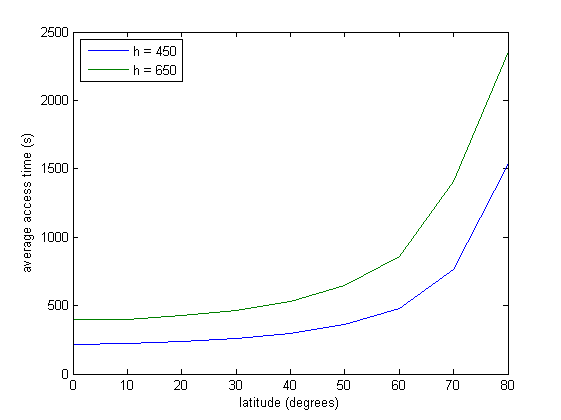
\includegraphics[width=1.0\textwidth]{Figures/accesstid450og650}
  \end{center}
  \caption[Accesstid for 450 og 650]{Access times for $h=450km$ and $h=650km$ as a function of ground station latitude}
  \label{fig:acctid}
\end{figure}

Since we don't know when the satellite will be launched we don't know the exact orbit. The project manager, Roger Birkeland, told us that the orbit will have $h\in (450km,650km)$ and $i=98$. The uncertainty in $h$ is critical, because the height above the earth dramatically changes the access time of a ground station, see Fig. \ref{acctid}. 

\begin{figure}
  \begin{center}
    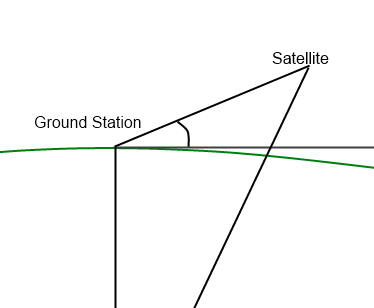
\includegraphics[width=0.7\textwidth]{Figures/groundstation_satelitte_geometry}
  \end{center}
  \caption[Ground station satellite geometry]{Illustration of geometry between a ground station and a satellite}
  \label{fig:gs_s_geom}
\end{figure}

A ground station can only communicate with a satelitte when it has a certain elevation. This elevation can differ from case to case depending on atmospheric effects, frequency and more. 
In the following we assume that the minimum elevation is 25 degrees, maximum elevation is 90 degrees and no constraints on the azimuth angle.  For a illustration see Fig. \ref{fig:gs_s_geom}.

\begin{figure}
  \begin{center}
    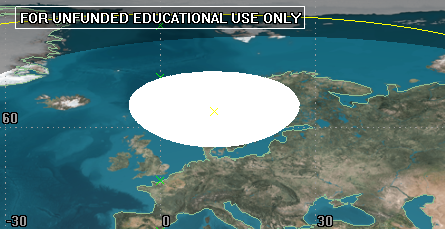
\includegraphics[width=0.8\textwidth]{Figures/ntnu_footprint}
  \end{center}
  \caption[ntnu footprint]{NTNU ground station range}
  \label{fig:ntnu_range}
\end{figure}

The result of this is that the ground station can communicate with the satelitte whenever the ground track is inside a rough circle centered on the ground station, see Fig. \ref{fig:ntnu_range} for the estimated "range" of the ground station at Gløshaugen operating with these constraints.

This ground station will on average be able to communicate with the satellite t seconds per day. That means that we will be able to download

\begin{equation}
D= d \cdot t
\end{equation}

where d is the bandwidth bandwidth available for transferring scientific data. $d$ is assumed to be 2.4 kbps. If the satellite has a orbit with $h=450km$ we can communicate with the satellite 540 seconds per day on average which gives 1.3 Mbit of data per day. If the satellite has a orbit with $h=650$ we can communicate 980 seconds on average, which gives 2.4 Mbit.
The amount of data we need to download per day is unknown, but the project manager told us 1 MB per day would be a good target. 



